\documentclass{article}
\PassOptionsToPackage{numbers,compress}{natbib}
\usepackage[dblblindworkshop]{neurips_2026}
\workshoptitle{AXIOM}
\usepackage[utf8]{inputenc}
\usepackage[T1]{fontenc}
\usepackage{hyperref}
\usepackage{url}
\usepackage{booktabs}
\usepackage{amsfonts,amsmath,amssymb}
\usepackage{nicefrac}
\usepackage{microtype}
\usepackage{graphicx}
\usepackage{xcolor}
\usepackage{caption}
\usepackage{tikz}\usepackage{enumitem}
\usetikzlibrary{arrows.meta,positioning,shapes.geometric,fit,calc}
\captionsetup{font=small,labelfont=bf,skip=3pt}
\setlength{\textfloatsep}{7pt}\setlength{\intextsep}{6pt}\setlength{\floatsep}{6pt}
\setlength{\abovedisplayskip}{3pt}\setlength{\belowdisplayskip}{3pt}\setlength{\abovedisplayshortskip}{2pt}\setlength{\belowdisplayshortskip}{2pt}
\makeatletter
\renewcommand\section{\@startsection{section}{1}{\z@}{-1.4ex \@plus -0.5ex \@minus -0.2ex}{0.7ex \@plus 0.2ex}{\large\bfseries\raggedright}}
\renewcommand\subsection{\@startsection{subsection}{2}{\z@}{-1.0ex \@plus -0.4ex \@minus -0.2ex}{0.5ex \@plus 0.1ex}{\normalsize\bfseries\raggedright}}
\renewcommand\paragraph{\@startsection{paragraph}{4}{\z@}{0.8ex \@plus 0.3ex \@minus 0.2ex}{-1em}{\normalsize\bfseries}}
\makeatother
\setlist{nosep}
\setlength{\parskip}{1pt plus 0.5pt}
\captionsetup{font=scriptsize}
\graphicspath{{../figs/}}

\title{Superposition Is Free to Quantize: Precision Cost Is Set by Outliers and Feature Margins, Not Feature Density}

\author{Anonymous Author(s)}

\begin{document}
\nolinenumbers
\maketitle

\begin{abstract}
A direction is only as resolvable as the grid it is stored on, so a layer that superposes more features per dimension
should need more bits. We preregistered
that hypothesis as a closed-form law (half a bit per doubling of features-per-dimension $F$) and tested it in 2{,}100
toy models, against five non-quantization damage families, and inside GPT-2 small. It is wrong:
the critical bit-width is flat in $F$ over a $14\times$ range (slope $-0.11$, CI $[-0.12,-0.09]$). What sets it is a
tolerance to relative weight perturbation that is independent of $F$ and shared within $2\times$ by rounding, dithering,
stochastic rounding and Gaussian noise, together with the outlier ratio $\kappa=\max|W|/\mathrm{rms}(W)$, entering as
$\log_2\kappa$: causally in the toy model ($R^2=0.92$), across GPT-2's 48 weight matrices ($R^2=0.53$; slope $0.6$--$0.7$, of
which a quantizer-free noise arm predicts $0.54$) and for their input activations (slope $1.12$ [$0.91$, $1.39$], $R^2=0.73$). In an exploratory follow-up the half-bit-per-doubling exponent reappears one level down: a feature's critical
bit-width follows its own fp32 margin, in the toy model ($R^2=0.68$), for GPT-2's next-token predictions (logit margin, not
rarity; $R^2=0.23$ per token, $0.90$ binned) and for 22{,}499 sparse-autoencoder features ($R^2=0.45$; $0.94$ binned):
quantization deletes a model's weakest features first, in an order a one-number statistic predicts. This yields a forecast from the fp32
model alone: margins predict which tokens a 4/5/6-bit model gets wrong (AUC 0.80/0.91/0.95; rarity 0.57), magnitudes predict which
SAE features are erased (AUC 0.87--0.94; frequency at chance), and the activation outlier ratio predicts which matrices need more
than 5 activation bits (AUC 0.97).
\end{abstract}

\section{Introduction}
Superposition, packing more features than dimensions as nearly orthogonal directions~\cite{elhage2022toy}, is the
prevailing account of how networks represent sparse features, and every quantitative treatment of it assumes
infinite-precision weights; quantization stores those weights on a coarse grid. The two have never been connected, yet a
connection is natural: a direction is only as resolvable as the grid it is stored on, so a layer
that superposes more features per dimension ($F$) should need more bits, an intuition entertained, without controls, in
the one prior experiment on the question~\cite{bitnets}. If true, it would convert a mechanistic quantity into an engineering one and give a representational account of the
weight-outlier counterpart of the folklore that outliers make layers hard to quantize~\cite{dettmers2022,xiao2023,lin2024awq}.

We made the intuition precise and \emph{preregistered} it (Section~\ref{sec:background}): $b_{\mathrm{crit}} = 1 +
\log_2(1+\kappa\sqrt{F/3})$, half a bit per doubling of $F$, with decision bands, controls and a real-model bridge committed
before any experiment ran. Our contributions:
\begin{itemize}\setlength\itemsep{2pt}
\item \textbf{The intuition is wrong.} Across 40 toy configurations spanning $F = 4$--$56$, under both
quantization-aware and post-training quantization, the critical bit-width is flat in $F$ (slope $-0.11$
[$-0.12$, $-0.09$]); in GPT-2 a superposition proxy predicts nothing ($R^2=0.04$). A corrected derivation explains why: at high $F$ added interference must be compared with existing interference, and $F$ cancels.
\item \textbf{What sets the bit-width.} A tolerance to relative weight perturbation that is independent of $F$ and
shared within $2\times$ by five damage families, and the outlier ratio $\kappa$, entering as $\log_2\kappa$: causally in the
toy model (clipping $\kappa$ moves $b_{\mathrm{crit}}$, $R^2=0.92$) and in GPT-2's 48 matrices ($R^2=0.53$). The tolerance grows
as $\kappa^{0.46}$ (measured with Gaussian noise, no quantizer), predicting an RTN slope of $0.54$ [$0.35$, $0.71$] against the
independently measured $0.63$ [$0.49$, $0.75$]. The same law holds for activations (post hoc): slope $1.12$ [$0.91$, $1.39$], $R^2=0.73$.
\item \textbf{A per-feature law (exploratory, not preregistered).} The half-bit-per-doubling exponent is real at the
feature level: a feature's critical bit-width follows its fp32 margin, in toy models ($R^2=0.68$), for GPT-2 next-token
predictions (margin beats rarity; $R^2=0.23$ per token, $0.90$ binned) and for GPT-2's internal sparse-autoencoder
features ($R^2=0.45$ per feature, $0.94$ binned, $n=22{,}499$). This is a candidate mechanism for the tail-loss phenomenon of compressed models~\cite{hooker2019,hooker2020}.
\end{itemize}

\begin{figure}[t]
\centering
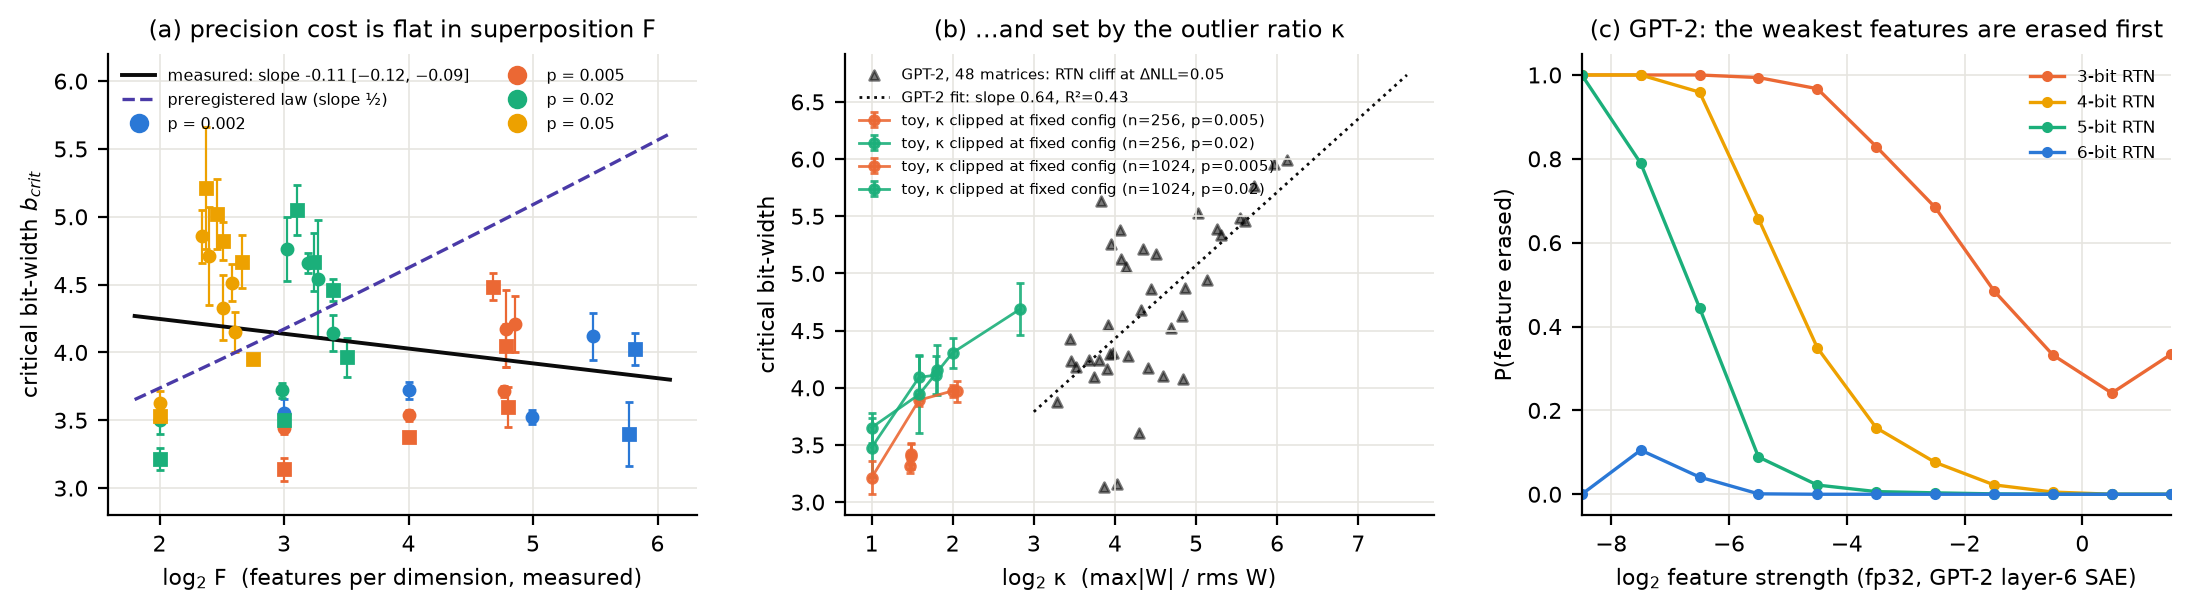
\includegraphics[width=0.66\linewidth]{fig_hero.png}
\caption{\textbf{Overview of the three main results.} \textbf{(a)} Critical bit-width (RTN, QAT, 95\,\% retention; mean $\pm$ SD over 4 seeds) against measured
features-per-dimension for the main sweep, with the preregistered law. \textbf{(b)} $b_{\mathrm{crit}}$ against
$\log_2\kappa$: toy models with $\kappa$ moved by weight clipping at fixed configuration, and GPT-2's 48 matrices (each
quantized alone, per-tensor RTN, threshold $\Delta\mathrm{NLL}=0.05$). \textbf{(c)} Fraction of GPT-2 layer-6
sparse-autoencoder features whose activation pattern is lost when blocks 0--5 are quantized jointly, by feature strength.}
\label{fig:hero}
\end{figure}

\paragraph{Related work.} Toy models of superposition established the phenomenon at infinite precision~\cite{elhage2022toy}; a
BitLinear replication reported ``later superposition onset'' without controls~\cite{bitnets}; our E1/E3 contradict the
resolution intuition behind both. Compression is known to hurt the
long tail~\cite{hooker2019,hooker2020}, outliers to govern quantization difficulty~\cite{dettmers2022,xiao2023,lin2024awq,frantar2022gptq},
and low-bit failures have architectural accounts~\cite{inputs2025}. We supply a mechanism at both levels: outlier ratios set a
layer's weight and activation bit budgets through an $F$-independent tolerance, and margins set which features go first.

\section{Background and the Preregistered Hypothesis}
\label{sec:background}

\subsection{Toy models of superposition}
We use the standard tied-weight toy model of superposition~\cite{elhage2022toy} (Figure~\ref{fig:pipeline}): $x\in\mathbb{R}^n$ with feature $i$ active
with probability $p$ and value $\sim U[0,1]$; $h=Wx$, $W\in\mathbb{R}^{m\times n}$; $\hat x=\mathrm{ReLU}(W^\top h+b)$;
squared-error loss with importance $I_i$. Writing $W_i$ for column $i$, $\hat x_i = \mathrm{ReLU}(\lVert W_i\rVert^2x_i +
\sum_{j\neq i}(W_i^\top W_j)x_j + b_i)$: the sum is the interference superposition costs. Per feature we measure
$\rho_i = 1-\nu_i/\nu_i^0$ ($\nu_i$ the reconstruction error, $\nu_i^0$ that of the best constant); a column is \emph{live} if $\lVert W_i\rVert\ge0.5$; $F = k/m$ with $k$ the live count of the fp32 model. Retention at
bit-width $b$ is $R(b) = \sum_{i\in\mathrm{live}}\rho_i(b)/\sum_{i\in\mathrm{live}}\rho_i(\infty)$ on identical samples,
and $b_{\mathrm{crit}}$ is the interpolated width at which $R = 0.95$ ($b=2$ never fitted).

\begin{figure}[t]
\centering
\scalebox{0.56}{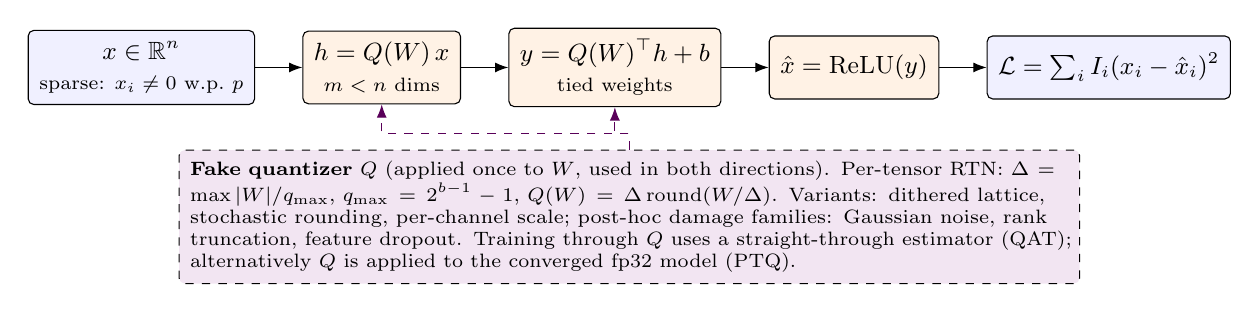
\begin{tikzpicture}[
  node distance=4mm and 6mm, >=Latex, font=\small,
  box/.style={draw, rounded corners=2pt, minimum height=8mm, inner sep=4pt, align=center},
  data/.style={box, fill=blue!6},
  op/.style={box, fill=orange!10},
  q/.style={box, fill=violet!10, dashed, text width=0.92\linewidth, align=left, font=\scriptsize}]
  \node[data] (x) {$x\in\mathbb{R}^n$\\ \scriptsize sparse: $x_i\ne0$ w.p.\ $p$};
  \node[op, right=of x] (W) {$h = Q(W)\,x$\\ \scriptsize $m<n$ dims};
  \node[op, right=of W] (Wt) {$y = Q(W)^{\top}h + b$\\ \scriptsize tied weights};
  \node[op, right=of Wt] (relu) {$\hat x = \mathrm{ReLU}(y)$};
  \node[data, right=of relu] (loss) {$\mathcal L=\sum_i I_i (x_i-\hat x_i)^2$};
  \draw[->] (x) -- (W); \draw[->] (W) -- (Wt); \draw[->] (Wt) -- (relu); \draw[->] (relu) -- (loss);
  \node[q, below=6mm of $(x.south west)!0.5!(loss.south east)$, anchor=north] (quant) {\textbf{Fake quantizer $Q$} (applied once to $W$, used in both directions). Per-tensor RTN: $\Delta = \max|W|/q_{\max}$, $q_{\max}=2^{b-1}-1$, $Q(W)=\Delta\,\mathrm{round}(W/\Delta)$. Variants: dithered lattice, stochastic rounding, per-channel scale; post-hoc damage families: Gaussian noise, rank truncation, feature dropout. Training through $Q$ uses a straight-through estimator (QAT); alternatively $Q$ is applied to the converged fp32 model (PTQ).};
  \draw[->, dashed, violet!70!black] (quant.north) -- ++(0,2mm) -| (W.south);
  \draw[->, dashed, violet!70!black] (quant.north) -- ++(0,2mm) -| (Wt.south);
\end{tikzpicture}}
\caption{\textbf{The toy model and the quantization pipeline.} A sparse feature vector is compressed through $W$ into $m<n$
dimensions and reconstructed with the same (tied) weights; the interference term $\sum_{j\ne i}(W_i^\top W_j)x_j$ is the price
of superposition. The fake quantizer $Q$ replaces $W$ in both directions; under QAT gradients pass through it with a
straight-through estimator, under PTQ it is applied once to a converged model. Every quantity used in the analysis is
measured on the resulting model.}
\label{fig:pipeline}
\end{figure}

The quantizer is per-tensor symmetric round-to-nearest (RTN), $q_{\max}=2^{b-1}-1$, $\Delta=\max|W|/q_{\max}$, applied
once to $W$ and used in both directions, trained through a straight-through estimator (QAT) or applied post-training (PTQ);
also dithered, stochastic-rounding and per-channel variants. The residual $\varepsilon = Q(W)-W$ is always measured.

\subsection{The preregistered law}
With unit live columns, tied weights double the cross-talk, only live columns interfere
(dead columns round to exactly 0), and $\max|W| = \kappa\,\mathrm{rms}(W)$ grows with occupancy. Summing the
quantization-induced cross-talk over $k$ live interferers active with probability $p$ gives an added interference
variance $p\kappa^2k^2/(18\,mn\,q_{\max}^2)$; equating it to the retention threshold $\nu^0/2$ and using $n\approx k$
yields $q_{\max,\mathrm{crit}} = \kappa\sqrt{F/3}$, i.e.\
\begin{equation}
b_{\mathrm{crit}} = 1+\log_2\!\big(1+\kappa\sqrt{F/3}\big) \approx \mathrm{const}+\tfrac12\log_2F .
\label{eq:law}
\end{equation}
The slope $\nicefrac12$ was the claim (bands: $[0.4,0.6]$ confirmed; $<0.15$ dead).

\subsection{Why the law fails}
Recorded after a sizing pilot and before the main sweep (Appendix~\ref{app:score}). The derivation
compares the \emph{added} interference with the explainable variance. But at $F\gg1$ the fp32 model already carries
interference many times that, the Welch bound gives $\sum_{j\neq i}(W_i^\top W_j)^2 \gtrsim F-1$, and survives it
through the ReLU with a strongly negative bias. The loss responds to added cross-talk \emph{relative to existing}
cross-talk: per pair $2\sigma_\varepsilon^2$ against $1/m$, a ratio $2m\sigma_\varepsilon^2 =
\lVert Q(W)-W\rVert_F^2/\lVert W\rVert_F^2 = \sigma_{\mathrm{rel}}^2$, the squared relative perturbation of each feature
direction. $F$ cancels. Since the residual lives on the live columns, $\sigma_{\mathrm{rel}} =
\kappa_{\mathrm{live}}/(\sqrt{12}q_{\max})$ with $\kappa_{\mathrm{live}} = \max|W|/\mathrm{rms}(W_{\mathrm{live}})$, so the
corrected prediction is $\sigma_{\mathrm{rel,crit}}$ independent of $F$ and
\begin{equation}
b_{\mathrm{crit}} \approx 1+\log_2\!\big(1+\kappa_{\mathrm{live}}/(\sqrt{12}\,\sigma_{\mathrm{rel,crit}})\big) = \mathrm{const} + \log_2\kappa_{\mathrm{live}} .
\label{eq:corrected}
\end{equation}
The algebra is the uniform-quantizer noise formula inverted; the empirical content is that $\sigma_{\mathrm{rel,crit}}$
does not depend on how densely features are packed.

\section{Methods}
\label{sec:methods}

Predictions, decision bands, fit rules and controls were committed before any experiment ran (design: Figure~\ref{fig:design},
appendix); every later analysis change is a dated deviation-log entry (D1--D4, Appendix~\ref{app:score}) written before the
affected results were inspected.



\subsection{Training, evaluation and controls}
All toy models: Adam $10^{-3}$, warm-up and cosine decay, 6000 steps, fp32; $\ge$40k evaluation samples with the quantizer
active; every arm of a (configuration, seed) shares data and evaluation samples (paired), and every mean carries a seed SD or
a seed-bootstrap CI. The
preregistered hard count $\#\{\rho_i\ge0.5\}$ is degenerate under uniform importance (all live features share nearly the
same $\rho$), so $R_{\mathrm{live}}$ is used with the hard count reported wherever defined. Seven damage families are applied
post hoc to the same fp32 models on the common axis $\sigma_{\mathrm{rel}} = \lVert D(W)-W\rVert_F/\lVert W\rVert_F$ with
the undamaged model evaluated inside every stack. GPT-2 small (124M, fp32, WikiText-2 held-out blocks, embeddings never
quantized): each of the 48 matrices is damaged alone with Gaussian noise and, separately, RTN; $\sigma_{\mathrm{crit}}$ is
the Gaussian-arm threshold and $b_{\mathrm{rtn}}$ the RTN-arm cliff, independent measurements, so predicting one from the
other through Eq.~\eqref{eq:corrected} is a test, not an identity. Joint experiments use per-channel scaling. Activations are quantized per matrix with per-tensor RTN ($\kappa_{\mathrm{act}} = \max|x|/\mathrm{rms}(x)$).
Full details in Appendix~\ref{app:methods}.

\section{Results}
\label{sec:results}
\subsection{The critical bit-width is flat in superposition}
 The main sweep ($m\in\{10,16\}$, $n/m\in\{4,\dots,128\}$, $p\in\{0.002,\dots,0.05\}$,
$b\in\{2,\dots,8,\infty\}$, 4 seeds, 1536 models) gives Figure~\ref{fig:hero}a (full plot: Figure~\ref{fig:money}, appendix): over 40 cells with $F = 4.0$--$56.5$
and $\kappa = 2.5$--$13.5$, $b_{\mathrm{crit}}$ is $3.1$--$5.2$ bits and its slope in $\log_2F$ is $-0.11$
[$-0.12$, $-0.09$]. Post-training RTN on the same
models: $3.87\pm0.15$ bits in every cell, slope $+0.03$ [$0.02$, $0.04$]. In GPT-2 small (48 matrices, one damaged
at a time, Appendix~\ref{app:methods}) the noise threshold has no relation to a superposition proxy $\hat F = d_{\mathrm{in}}/\mathrm{PR}$
(slope $+0.14$ [$-0.13$, $0.35$], $R^2=0.04$).

\subsection{An $F$-independent tolerance to perturbation}
 Applying seven damage families post-hoc to the same fp32 models on a common axis
$\sigma_{\mathrm{rel}} = \lVert D(W)-W\rVert_F/\lVert W\rVert_F$: RTN, per-channel RTN, dithered and stochastic rounding
and Gaussian noise all cost 5\,\% of the represented features' explained variance at $\sigma_{\mathrm{rel}}\approx
0.10$--$0.23$, flat in $F$ (slopes $0.00$--$0.05$ against the predicted $-\nicefrac12$; 44 cells; Figure~\ref{fig:e3}, appendix). Structured damage behaves differently (dropout tolerated to $0.3$--$0.5$; rank truncation catastrophic).

\subsection{Outliers set the bit-width, and a non-circular test of the slope}
 Across the sweep $b_{\mathrm{crit}} = 2.0+0.72\log_2\kappa$ ($R^2 = 0.82$;
$b_{\mathrm{crit}}-\log_2\kappa = 1.99\pm0.31$). To break the collinearity of $\kappa$ with the live fraction we moved $\kappa$ directly: clipping weights at $c\cdot\mathrm{rms}(W)$ at fixed $(m,n,p)$ takes $\kappa$ from $7.1$ to $2.0$ and
$b_{\mathrm{crit}}$ from $4.69$ to $3.65$; pooled within-cell slope $0.65$, $R^2=0.92$ (Figure~\ref{fig:hero}b; Figure~\ref{fig:kappa}, appendix).
In GPT-2 the independently measured per-tensor RTN cliff of each matrix follows $\log_2\kappa$ with slope $0.63$
[$0.49$, $0.76$], $R^2 = 0.53$, against $R^2=0.14$ for $\hat F$, and
converting each matrix's Gaussian-noise threshold to bits with Eq.~\eqref{eq:corrected} reproduces its RTN cliff with a
mean error of $-0.23$ bits. The slope is $0.6$--$0.7$ in all three settings; a non-circular test of why: $\sigma_{\mathrm{crit}}$ is
measured from the Gaussian-noise arm and involves no quantizer, and across the GPT-2 matrices it grows with the outlier
ratio, $\sigma_{\mathrm{crit}}\propto\kappa^{e}$ with $e = 0.46$ [$0.29$, $0.65$] ($R^2=0.35$). Substituted into
Eq.~\eqref{eq:corrected} this predicts an RTN slope of $1-e = 0.54$ [$0.35$, $0.71$]; the slope measured independently
from the RTN arm is $0.63$ [$0.49$, $0.75$], a paired difference of $+0.09$ [$-0.05$, $+0.26$] (replicated at $\Delta\mathrm{NLL}=0.02$, Appendix~\ref{app:methods}):
consistent within error, central value $0.1$ low, so the account explains part of the shortfall, not all. $\sigma^*$ is
not a constant but a smooth function of $\kappa$ that is flat in $F$. With per-channel scaling the pathology
disappears and every GPT-2 matrix crosses the threshold at $2.70\pm0.33$ bits, uncorrelated with $\kappa$ or $\hat F$;
consequently mixed precision has little left to gain: uniform per-channel RTN is within $0.01$--$0.02$ nats of a
sensitivity oracle at 4 and 5 bits, and a $\kappa$-based allocation is \emph{worse} than uniform there (Appendix~\ref{app:methods},
Table~\ref{tab:mixed}). Dithered quantization is \emph{worse} than the shared lattice ($+0.27\pm0.13$ bits under QAT) because it moves
the exact zeros of dead columns off the lattice; stochastic rounding is worse still ($+0.63\pm0.11$).

\subsection{Activation quantization (post hoc)}
For each matrix alone, its input activations are quantized with per-tensor RTN; $\kappa_{\mathrm{act}}$ ranges from $10$ to $382$. The activation
$b_{\mathrm{crit}}$ ($\Delta\mathrm{NLL}=0.05$; 42 of 48 interpolable) follows $\log_2\kappa_{\mathrm{act}}$ with slope
$1.12$ [$0.91$, $1.39$], $R^2=0.73$ (Figure~\ref{fig:act}, appendix), whereas the weight $\kappa$ of the same matrix does not predict it
($R^2=0.12$). The naive slope of $1$ holds for activations.

\subsection{Which features die first: the per-feature law (exploratory)}
 Under power-law importance $I_i=(i+1)^{-\alpha}$ the toy model drops features
from the tail, and quantization respects the order (prefix fraction unchanged, $0.95$--$0.99$). The ten most important features need 3 bits in every configuration, the marginal ones 4--8; across all 4{,}290
live features the critical bit-width follows the feature's fp32 margin above the retention threshold, $b_i = c -
0.52\log_2(\rho_i^{\mathrm{fp32}}-\tfrac12)$, $R^2 = 0.68$. The same law holds inside GPT-2 twice. For next-token
predictions (all matrices quantized jointly, per-channel RTN): at 4 bits, tokens with an fp32
logit margin below $\nicefrac18$ flip 58\,\% of the time, margin 1--2 logits 9\,\%, margin above 8 logits 0.5\,\%; the
critical bit-width falls with $\log_2$ margin at slope $-0.34$ per token ($R^2=0.23$; individual tokens are noisy) and
$-0.39$ for the binned means ($R^2=0.90$), and margin dominates rarity
($b_t = 5.30-0.36\log_2\mathrm{margin}-0.09\log_2\mathrm{freq}$). For internal features, using a public sparse autoencoder on the residual stream entering block 6 and quantizing
blocks 0--5 jointly: 26/84/99\,\% of the 22{,}499 live features survive 3/4/5 bits, and which ones are erased is set by their
strength (Figure~\ref{fig:hero}c; Figure~\ref{fig:sae}, appendix), features contributing $2^{-7}$ of the residual rms need $5.5$--$6$ bits, features at
$2^{0}$ survive at 3; per-feature slope $-0.37$ [$-0.38$, $-0.37$] ($R^2 = 0.45$ per feature, $0.94$ binned), with
frequency adding nothing ($+0.02$). Gaussian noise gives the same curves in every case.

\paragraph{Forecasting quantization damage from the fp32 model.} The law is usable before quantizing anything: fp32 margin
predicts which correct predictions a 4/5/6-bit model flips with ROC AUC $0.80$/$0.91$/$0.95$ (rarity: $0.60$/$0.56$/$0.57$); fp32
magnitude predicts which SAE features are erased at 3/4/5 bits with AUC $0.87$/$0.91$/$0.94$ (frequency: at or below chance); the
toy margin predicts which features need more than 4 bits with AUC $0.92$; the activation outlier ratio predicts which matrices need
more than 5 activation bits with AUC $0.97$ (weight $\kappa$: $0.64$). None of this requires running the quantized model.




\section{Conclusion}

Table~\ref{tab:key} (appendix) collects the numbers; the $\kappa$ law is the uniform-quantizer noise formula inverted; its content is that $\sigma^*$ does not depend on
how densely features are packed, so a layer's bit budget is fixed by its outliers and outlier suppression buys
$\log_2(\kappa_{\mathrm{before}}/\kappa_{\mathrm{after}})$ bits, up to the $\kappa^{0.46}$ compensation we measure.
Limitations: one tied toy layer with uniform importance in the main sweep; $\sigma^*$ is $F$-independent but its value
depends on architecture and loss criterion; one 124M model, one corpus, one SAE layer, post-training only, untested
at scale and under joint weight-plus-activation quantization. Weight bits need the $\sigma^*(\kappa)$ correction (slope $0.63$) while activation bits follow
$\kappa_{\mathrm{act}}$ with slope $1.12$ and no visible co-variation; we cannot yet explain the difference. The per-feature law and the activation arm are exploratory (Appendix~\ref{app:score}). In short: superposition is free to quantize, bits are set by outliers, and a model loses its weakest features first, predictably.

\begin{thebibliography}{9}\small
\bibitem{elhage2022toy} N.~Elhage et al. Toy models of superposition. \emph{Transformer Circuits Thread}, 2022.
\bibitem{hooker2019} S.~Hooker, A.~Courville, G.~Clark, Y.~Dauphin, A.~Frome. What do compressed deep neural networks forget? arXiv:1911.05248, 2019.
\bibitem{hooker2020} S.~Hooker, N.~Moorosi, G.~Clark, S.~Bengio, E.~Denton. Characterising bias in compressed models. arXiv:2010.03058, 2020.
\bibitem{dettmers2022} T.~Dettmers, M.~Lewis, Y.~Belkada, L.~Zettlemoyer. LLM.int8(): 8-bit matrix multiplication for transformers at scale. \emph{NeurIPS}, 2022.
\bibitem{xiao2023} G.~Xiao, J.~Lin, M.~Seznec, H.~Wu, J.~Demouth, S.~Han. SmoothQuant. \emph{ICML}, 2023.
\bibitem{lin2024awq} J.~Lin et al. AWQ: activation-aware weight quantization for LLM compression and acceleration. \emph{MLSys}, 2024.
\bibitem{frantar2022gptq} E.~Frantar, S.~Ashkboos, T.~Hoefler, D.~Alistarh. GPTQ. arXiv:2210.17323, 2022.
\bibitem{inputs2025} Why do some inputs break low-bit LLM quantization? arXiv:2506.12044, 2025.
\bibitem{bitnets} Toy models of superposition: what about BitNets? \emph{LessWrong}, 2024.
\bibitem{bloom2024sae} J.~Bloom. Open source sparse autoencoders for all residual stream layers of GPT-2 small. 2024.
\end{thebibliography}

\appendix
\begin{table}[h]\centering\footnotesize
\caption{Key results (CIs: seed bootstrap for toy models, matrix bootstrap for GPT-2; ``prereg.'' = preregistered value;
``P2 form'' = P2's functional form applied post hoc to a new arm; exploratory rows were not preregistered).}
\label{tab:key}
\setlength{\tabcolsep}{4pt}
\resizebox{\linewidth}{!}{\begin{tabular}{llll}\toprule
question & quantity & result & prereg.\\\midrule
does $F$ set bits? & $b_{\mathrm{crit}}$ slope in $\log_2F$, QAT / PTQ & $-0.11$ [$-0.12,-0.09$] / $+0.03$ [$0.02,0.04$] & $+0.5$\\
does $\kappa$ set bits? & within-cell slope in $\log_2\kappa$, $\kappa$ clipped (E6) & $0.65$, $R^2=0.92$ & $1$\\
 & GPT-2 RTN cliff vs $\log_2\kappa$ / vs $\log_2\hat F$ & $0.63$, $R^2=0.53$ / $0.28$, $R^2=0.14$ & --\\
 & GPT-2 activation bits vs $\log_2\kappa_{\mathrm{act}}$ / vs $\log_2\kappa_w$ (post hoc) & $1.12$ [$0.91,1.39$], $R^2=0.73$ / $0.35$, $R^2=0.12$ & P2 form\\
$F$-independent tolerance? & $\sigma_{\mathrm{rel,crit}}$ slope in $\log_2F$, five noise families & $0.00$ to $0.05$ & $-0.5$\\
which features die? (exploratory) & toy: $b_i$ vs $\log_2$ margin ($n=4290$) & $-0.52$, $R^2=0.68$ & --\\
 & GPT-2 tokens: $b_t$ vs $\log_2$ logit margin & $-0.34$ ($R^2$ 0.23 per token; $-0.39$, 0.90 binned) & --\\
 & GPT-2 SAE features: $b_f$ vs $\log_2$ strength ($n=22499$) & $-0.37$ [$-0.38,-0.37$] ($R^2$ 0.45; 0.94 binned) & --\\\bottomrule
\end{tabular}}
\end{table}
\begin{table}[h]\centering\small
\caption{Mixed precision on GPT-2 small: $\Delta$NLL (nats, held-out) at equal parameter-weighted average bits.}
\label{tab:mixed}
\begin{tabular}{lccccc}\toprule
avg.\ bits & uniform & $\kappa$-rule & noise-probe law & oracle & random ($\times3$)\\\midrule
3.5 & -- & 3.56 & \textbf{1.86} & 2.08 & 3.6--4.1\\
4.0 & \textbf{0.449} & 0.659 & 0.600 & 0.459 & 0.68--0.88\\
4.5 & -- & 0.274 & \textbf{0.190} & 0.183 & 0.26--0.33\\
5.0 & \textbf{0.084} & 0.094 & 0.103 & 0.067 & 0.10--0.11\\\bottomrule
\end{tabular}
\end{table}
\section{Preregistration scoring and dated deviations}
\label{app:score}
\begin{center}\small
\resizebox{\linewidth}{!}{\begin{tabular}{p{4.6cm}p{3.6cm}p{5.6cm}}\toprule
prediction & rule & outcome\\\midrule
P1: slope $\nicefrac12$ in $\log_2F$ & $[0.4,0.6]$ / $[0.15,0.35]$ / $<0.15$ & \textbf{dead}: $-0.11$ (QAT), $+0.03$ (PTQ), all definitions $<0.15$\\
P2: $\kappa$ enters as $\log_2\kappa$, slope 1 & $[0.7,1.3]$ / $\approx0$ / partial & \textbf{partial, strong}: $0.65$ ($R^2$ 0.92), $0.72$, $0.63$\\
P3: ordering preserved (power-law $I$) & prefix drop $<0.10$ & \textbf{confirmed}: $\le0.03$\\
E3: noise-like slope $-\nicefrac12$; structured $\approx0$ & & noise-like $\approx0$; dropout $+0.24$; rank catastrophic\\
E4: top features unchanged & drop $<0.05$ & tilt, not translation (uniform $I$)\\
LM: $\log_2\sigma_{\mathrm{crit}}$ vs $\log_2\hat F\in[-0.65,-0.35]$ & & \textbf{not}: $+0.14$ [$-0.13$, $0.35$]\\
D2 (pre-E1): $\sigma_{\mathrm{crit}}$ flat, $b=\mathrm{const}+\log_2\kappa$ & & \textbf{confirmed}\\\bottomrule
\end{tabular}}
\end{center}
Deviations (dated in the repository): D1, after the fp32-only gate, the hard count made continuous; D2, after the sizing
pilot and before the main sweep, the corrected derivation and its decision rule; D3, after a pilot damage run, clipping
bias and dead-feature accounting fixed by $R_{\mathrm{live}}$ with paired evaluation; D4, after an external review of the
draft, the activation arm added as a post-hoc application of P2's functional form to a new quantity (not preregistered
coverage), and the per-token and SAE analyses recorded as exploratory.

\section{Methods details}
\label{app:methods}
\paragraph{Training, evaluation and metrics.}
All toy models: Adam $10^{-3}$, 200-step warm-up, cosine decay, 6000 steps, fp32 on Apple MPS; $\ge$40k evaluation
samples with the quantizer active; every arm of a (configuration, seed) shares data and evaluation samples (paired), and
every mean carries a seed SD or a seed-bootstrap CI. Batched training of $K$ models per group uses per-model tensors for $p$,
bit-width and quantizer mode; $\kappa$ plateaus by step $\sim$4000. Per feature we record $\rho_i$, the column norm, $D_i$, $\kappa$ and the measured residual. An fp32 trust gate (E0, $n=400$, $m=30$) reproduces the
feature-dimensionality ladder (Figure~\ref{fig:e0}). The preregistered hard count $\#\{\rho_i\ge0.5\}$ is degenerate under
uniform importance (the model represents all live features with nearly identical $\rho$, so the count is a cliff and
seed-noisy); $R_{\mathrm{live}}$ is its continuous analogue, with the hard count reported wherever defined
(Appendix~\ref{app:score}).

\paragraph{Damage families (E3) and GPT-2 experiments.} Per-tensor mixed precision is not viable at these budgets: joint per-tensor damage is super-additive ($+4.6$ nats at 6 bits vs $1.6$ summed over single matrices; still $+0.14$ at 8 bits).
Seven damage families are applied post hoc to the same fp32 models on the common axis $\sigma_{\mathrm{rel}} = \lVert D(W)-W\rVert_F/\lVert W\rVert_F$:
RTN, dithered, stochastic rounding, per-channel RTN, Gaussian noise, rank truncation, feature dropout; the undamaged model
is evaluated inside every stack (paired). $\sigma_{\mathrm{rel,crit}}$ is $1.26\times$ larger at $m=16$ than at $m=10$
($\sqrt{16/10}$), as expected if the dominant damage is to each feature's own direction rather than cross-talk.
GPT-2 small (124M, fp32, WikiText-2 held-out blocks, embeddings never quantized): each of the 48 matrices is damaged alone with
Gaussian noise on a log grid and, separately, RTN at 3--6 bits ($\Delta$NLL on 49k tokens, residual stream cached up to the
damaged block); $\kappa$ and $\hat F=d_{\mathrm{in}}/\mathrm{PR}$ (participation ratio of the input covariance) per matrix.
$\sigma_{\mathrm{crit}}$ is the Gaussian-arm threshold and $b_{\mathrm{rtn}}$ the RTN-arm cliff: independent measurements,
so predicting one from the other through Eq.~\eqref{eq:corrected} is a test, not an identity. Per-tensor RTN on the three
$\kappa\approx160$--$190$ matrices is pathological (non-monotone in bits; joint damage $3\times$ super-additive), so all
joint experiments use per-channel scaling. Activation arm: each matrix's input activations quantized alone with per-tensor RTN
(absmax scale over the calibration tokens) at 3--8 bits, with $\kappa_{\mathrm{act}} = \max|x|/\mathrm{rms}(x)$. Tokens:
per-token fp32 logit margin and survival under joint quantization. SAE: \texttt{jbloom/GPT2-Small-SAEs-Reformatted} at
\texttt{blocks.6.hook\_resid\_pre} on the mean-centred residual with the decoder bias subtracted (84\,\% variance explained,
$L_0\approx58$), 196{,}596 tokens in 128-token BOS-prefixed contexts, $\rho_f = 1-\sum_t(a_f^q-a_f^{\mathrm{fp32}})^2/\sum_t(a_f^{\mathrm{fp32}})^2$,
live if firing on $\ge20$ tokens. Compute: about four GPU-hours on one laptop.


\section{Experimental design and additional figures}
\begin{figure}[h]
\centering
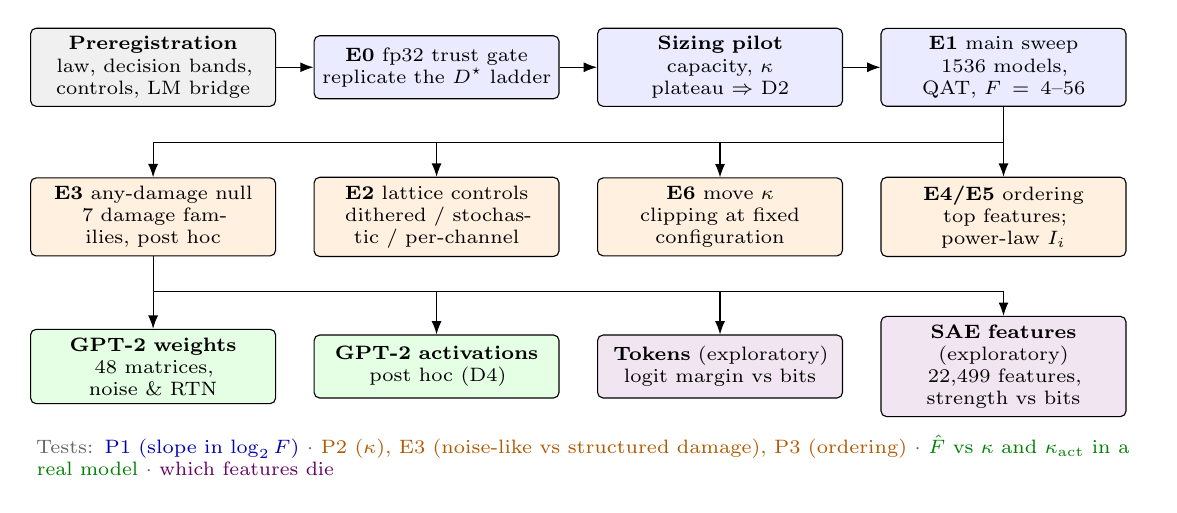
\begin{tikzpicture}[
  >=Latex, font=\scriptsize,
  st/.style={draw, rounded corners=2pt, minimum height=8mm, inner sep=3pt, align=center, text width=29mm},
  pre/.style={st, fill=gray!12}, exp/.style={st, fill=blue!8}, ctl/.style={st, fill=orange!12}, lm/.style={st, fill=green!10}, ex/.style={st, fill=violet!10}]
  \node[pre] (prereg) at (0,0) {\textbf{Preregistration}\\ law, decision bands, controls, LM bridge};
  \node[exp] (e0) at (3.6,0) {\textbf{E0} fp32 trust gate\\ replicate the $D^\star$ ladder};
  \node[exp] (pilot) at (7.2,0) {\textbf{Sizing pilot}\\ capacity, $\kappa$ plateau $\Rightarrow$ D2};
  \node[exp] (e1) at (10.8,0) {\textbf{E1} main sweep\\ 1536 models, QAT, $F=4$--$56$};
  \node[ctl] (e3) at (0,-1.9) {\textbf{E3} any-damage null\\ 7 damage families, post hoc};
  \node[ctl] (e2) at (3.6,-1.9) {\textbf{E2} lattice controls\\ dithered / stochastic / per-channel};
  \node[ctl] (e6) at (7.2,-1.9) {\textbf{E6} move $\kappa$\\ clipping at fixed configuration};
  \node[ctl] (e5) at (10.8,-1.9) {\textbf{E4/E5} ordering\\ top features; power-law $I_i$};
  \node[lm] (lmw) at (0,-3.8) {\textbf{GPT-2 weights}\\ 48 matrices, noise \& RTN};
  \node[lm] (lma) at (3.6,-3.8) {\textbf{GPT-2 activations}\\ post hoc (D4)};
  \node[ex] (tok) at (7.2,-3.8) {\textbf{Tokens} (exploratory)\\ logit margin vs bits};
  \node[ex] (sae) at (10.8,-3.8) {\textbf{SAE features} (exploratory)\\ 22{,}499 features, strength vs bits};
  \draw[->] (prereg) -- (e0); \draw[->] (e0) -- (pilot); \draw[->] (pilot) -- (e1);
  \draw (e1.south) -- ++(0,-0.45) coordinate (bus1); \draw (bus1) -- (bus1 -| e3.north);
  \foreach \n in {e3,e2,e6,e5} { \draw[->] (bus1 -| \n.north) -- (\n.north); }
  \draw (e3.south) -- ++(0,-0.45) coordinate (bus2); \draw (bus2) -- (bus2 -| sae.north);
  \foreach \n in {lmw,lma,tok,sae} { \draw[->] (bus2 -| \n.north) -- (\n.north); }
  \node[font=\scriptsize, text=black!60, anchor=north west, text width=14cm] at (-1.6,-4.55) {Tests: \textcolor{blue!70!black}{P1 (slope in $\log_2F$)} $\cdot$ \textcolor{orange!70!black}{P2 ($\kappa$), E3 (noise-like vs structured damage), P3 (ordering)} $\cdot$ \textcolor{green!50!black}{$\hat F$ vs $\kappa$ and $\kappa_{\mathrm{act}}$ in a real model} $\cdot$ \textcolor{violet!80!black}{which features die}};
\end{tikzpicture}
\caption{\textbf{Experimental design.} Grey: preregistration. Blue: the trust gate, the sizing pilot and the preregistered
main sweep. Orange: the controls that decide whether the result is about quantization, about outliers, and about which
features are lost. Green: the real-model bridge on GPT-2 weights and activations. Violet: exploratory per-feature analyses.}
\label{fig:design}
\end{figure}
\begin{figure}[h]\centering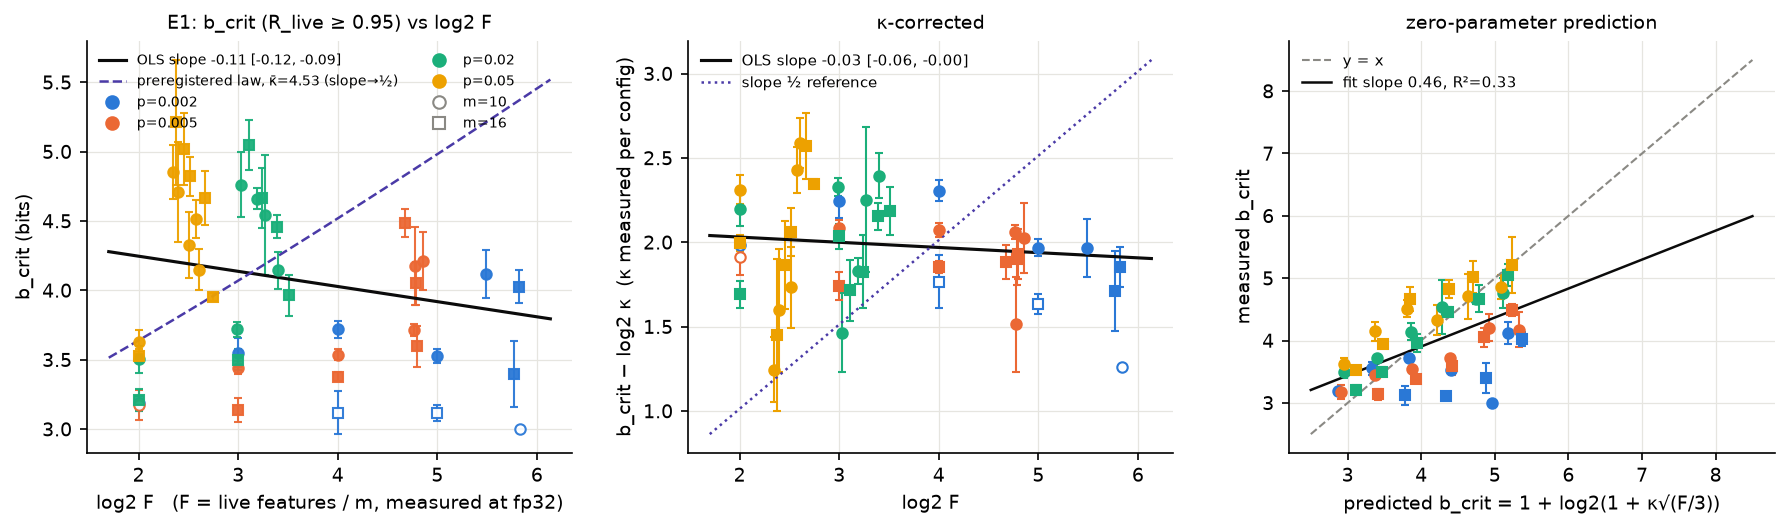
\includegraphics[width=\linewidth]{fig1_bcrit_vs_F_R_live_95.png}
\caption{The preregistered test (E1): $b_{\mathrm{crit}}$ against $\log_2F$ (left), $\kappa$-corrected (middle), zero-parameter prediction (right).}\label{fig:money}\end{figure}
\begin{figure}[h]\centering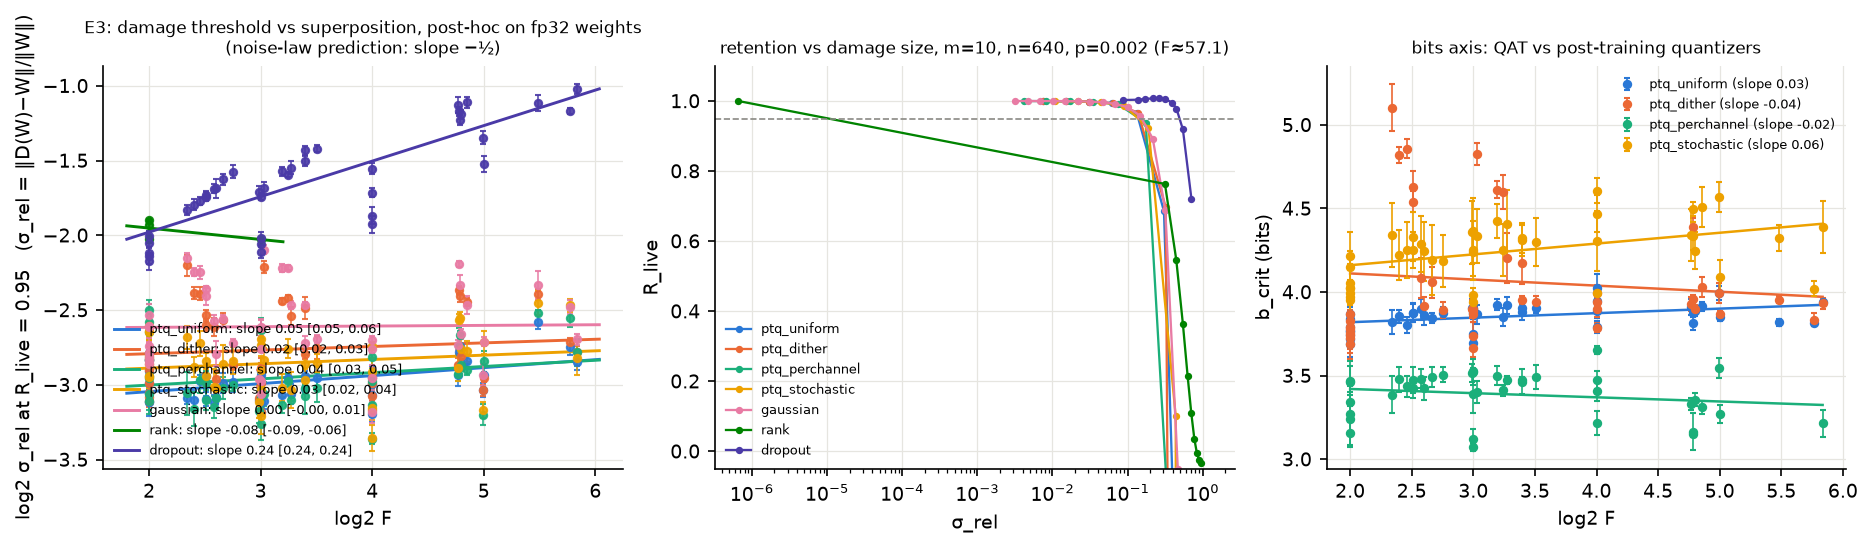
\includegraphics[width=\linewidth]{fig3_anydamage_null.png}
\caption{Any-damage null (E3): threshold vs $\log_2F$ for seven families; retention vs $\sigma_{\mathrm{rel}}$; bits axis.}\label{fig:e3}\end{figure}
\begin{figure}[h]\centering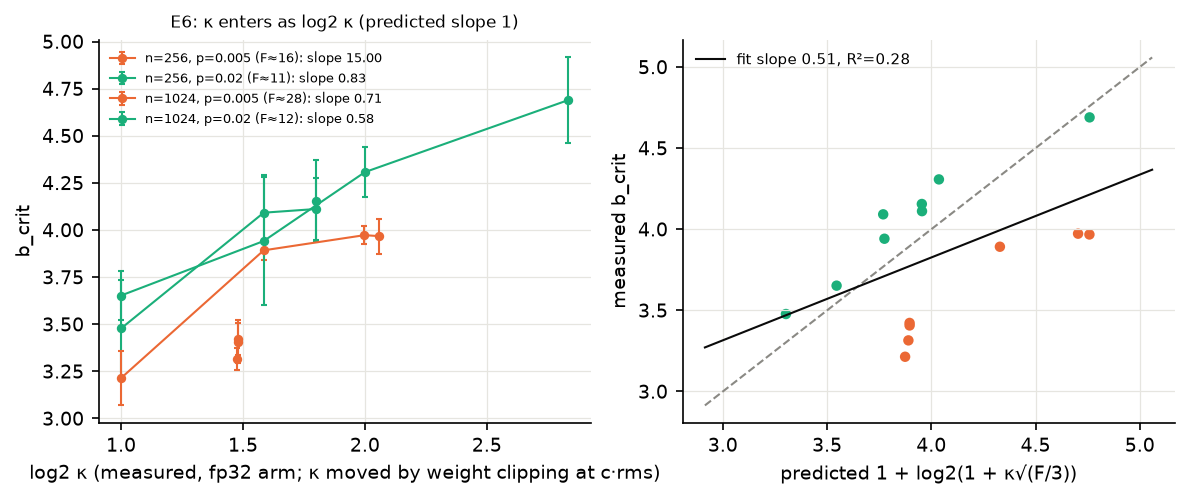
\includegraphics[width=0.8\linewidth]{fig8_kappa.png}
\caption{E6: $b_{\mathrm{crit}}$ against $\log_2\kappa$ with $\kappa$ moved by clipping at fixed configuration.}\label{fig:kappa}\end{figure}
\begin{figure}[h]\centering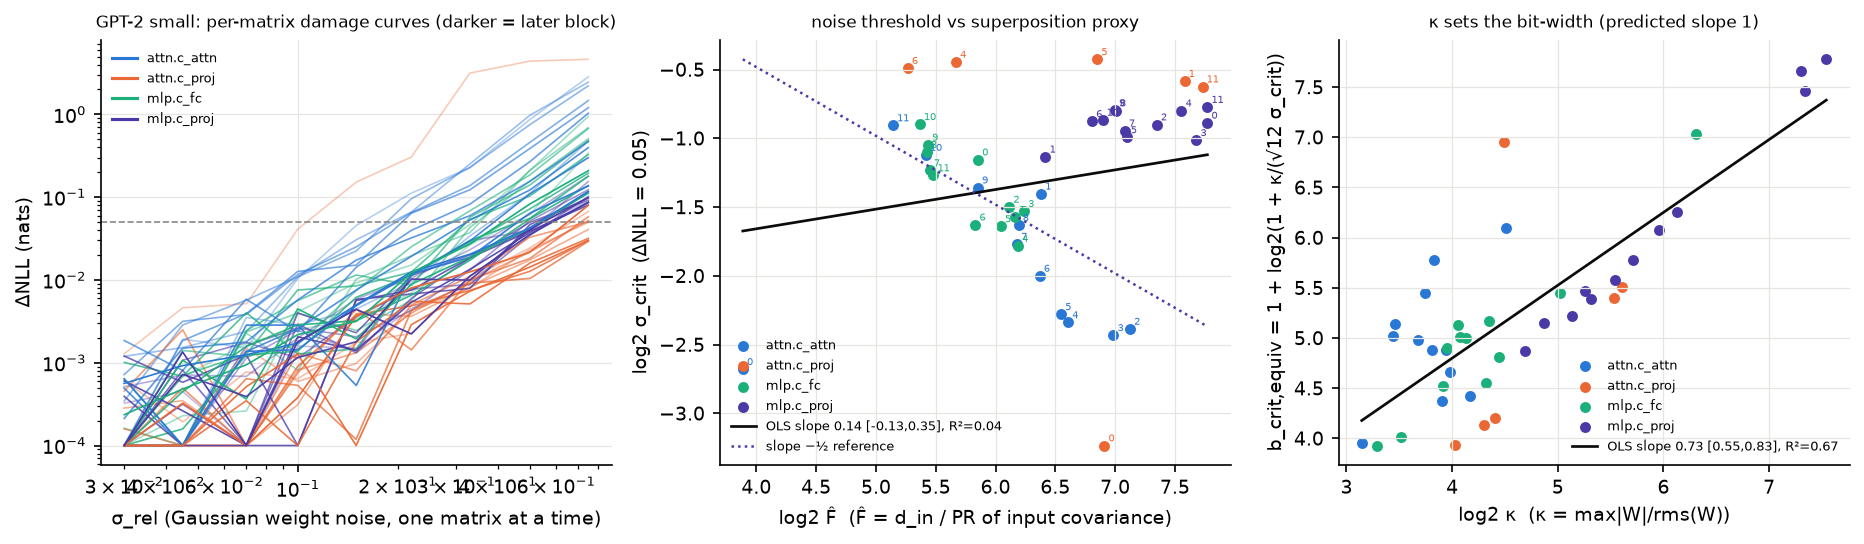
\includegraphics[width=\linewidth]{fig7_lm_layers.png}
\caption{GPT-2 per-matrix damage curves, noise threshold vs $\hat F$, bit-equivalent vs $\kappa$.}\label{fig:lm}\end{figure}
\begin{figure}[h]\centering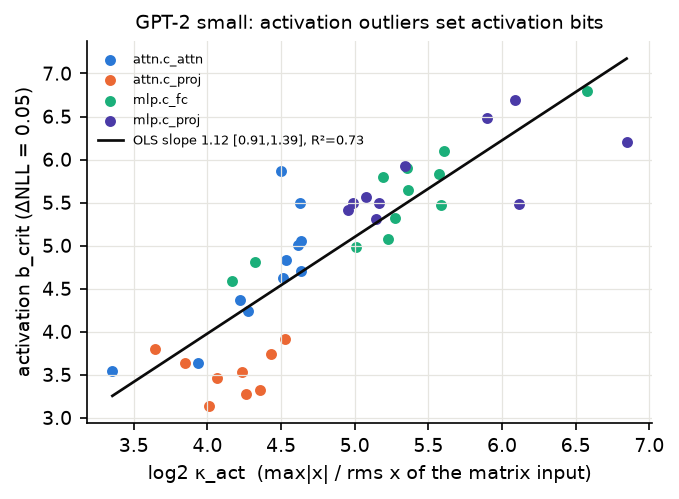
\includegraphics[width=0.55\linewidth]{fig12_activation_kappa.png}
\caption{Activation quantization (post hoc, D4): activation bit-width vs activation outlier ratio.}\label{fig:act}\end{figure}
\begin{figure}[h]\centering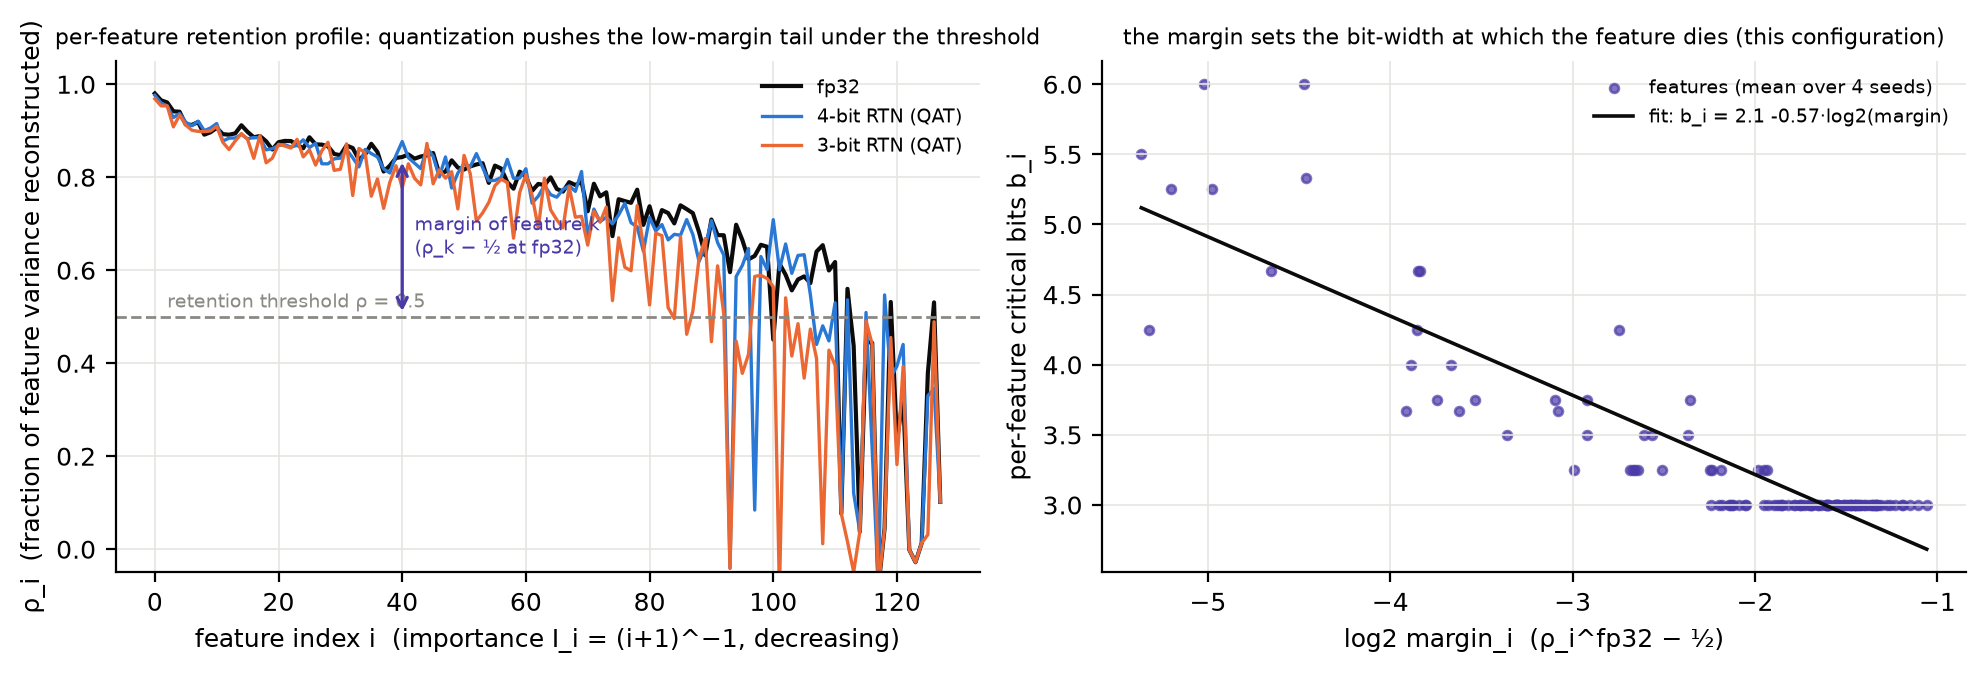
\includegraphics[width=\linewidth]{fig13_margin_concept.png}
\caption{The per-feature margin on one configuration: $\rho$ profiles and per-feature critical bits vs margin.}\label{fig:margin}\end{figure}
\begin{figure}[h]\centering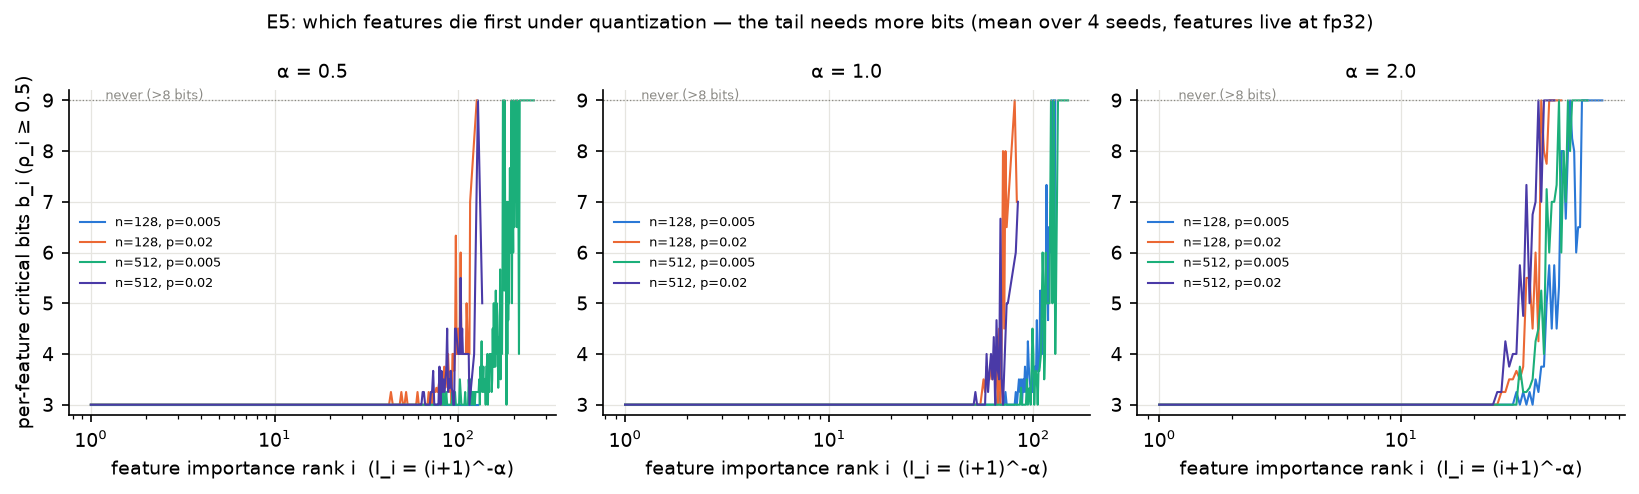
\includegraphics[width=\linewidth]{fig6b_per_feature_bits.png}
\caption{E5: per-feature critical bits against importance rank.}\label{fig:perfeature}\end{figure}
\begin{figure}[h]\centering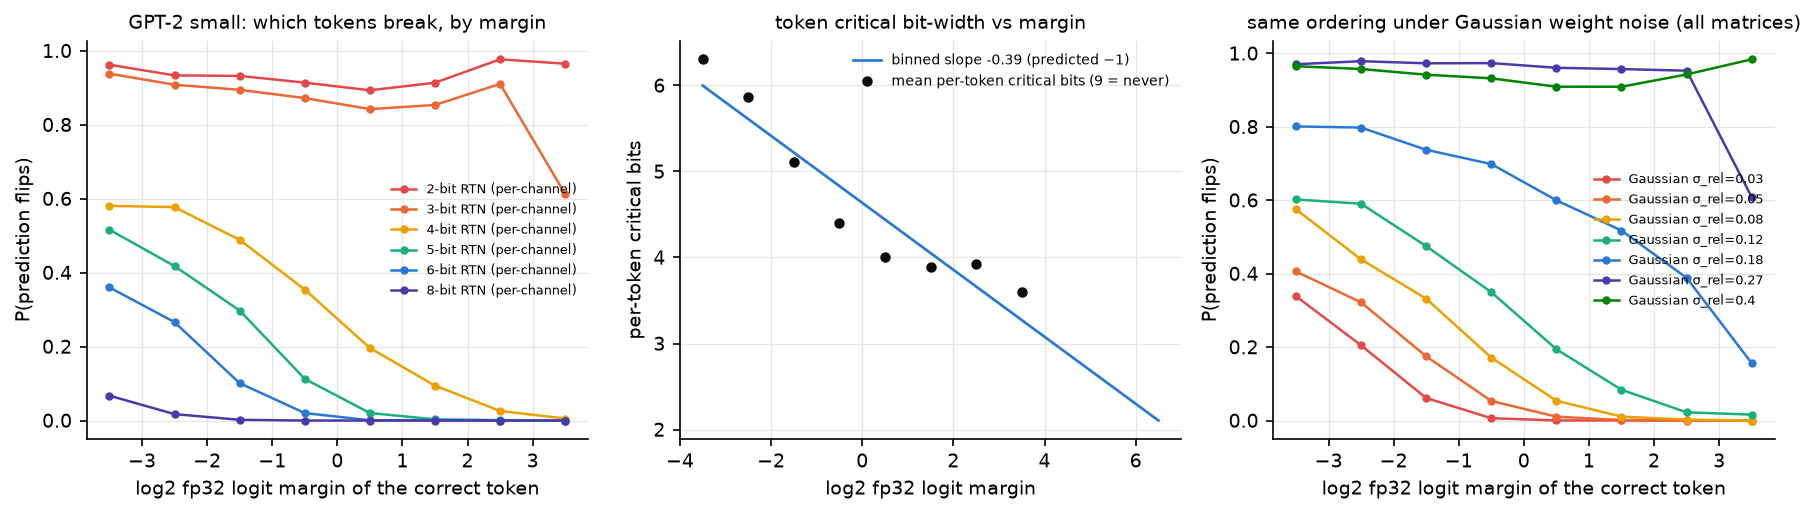
\includegraphics[width=\linewidth]{fig10_token_margins.png}
\caption{GPT-2 tokens: flip probability by margin, critical bits vs margin, Gaussian control.}\label{fig:tokens}\end{figure}
\begin{figure}[h]\centering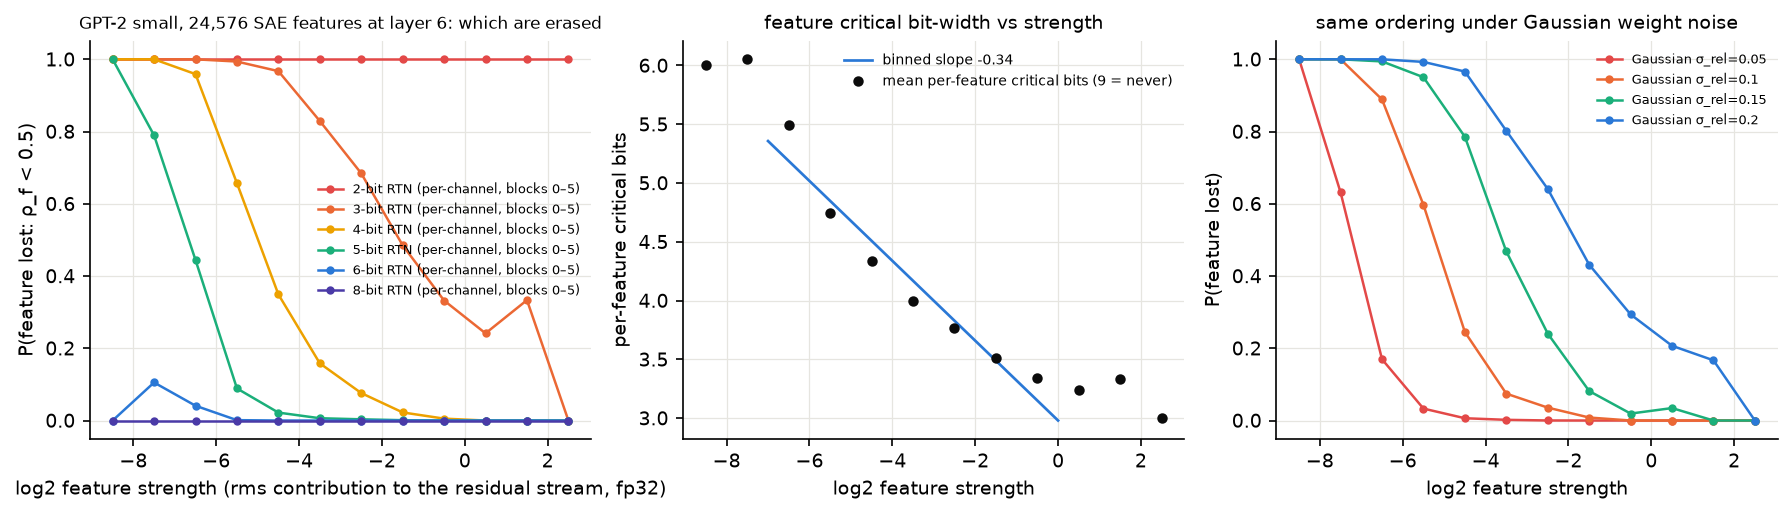
\includegraphics[width=\linewidth]{fig11_sae_features.png}
\caption{GPT-2 SAE features: loss by strength, critical bits vs strength, Gaussian control.}\label{fig:sae}\end{figure}
\begin{figure}[h]\centering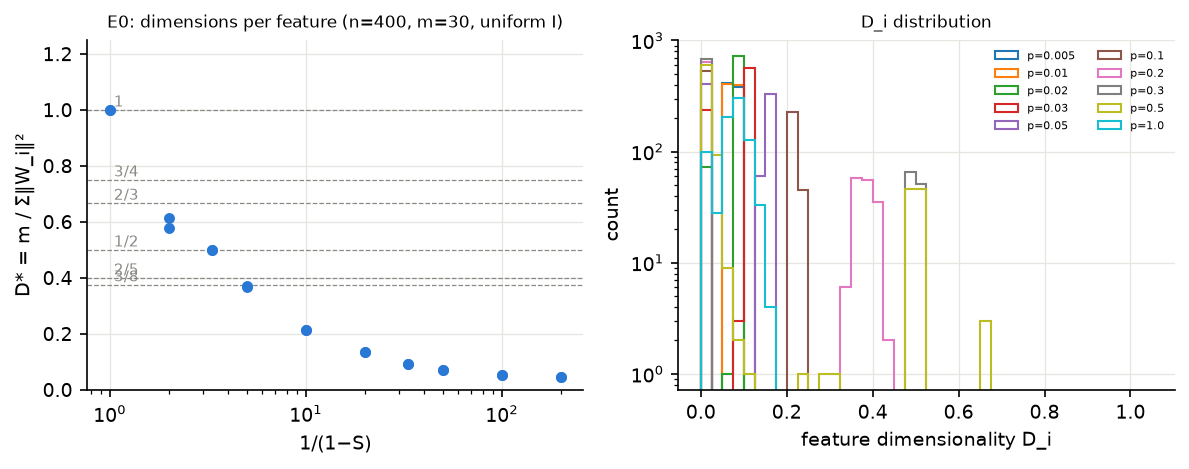
\includegraphics[width=0.85\linewidth]{fig0_e0_replication.png}
\caption{E0: fp32 replication of the feature-dimensionality ladder.}\label{fig:e0}\end{figure}
\begin{figure}[h]\centering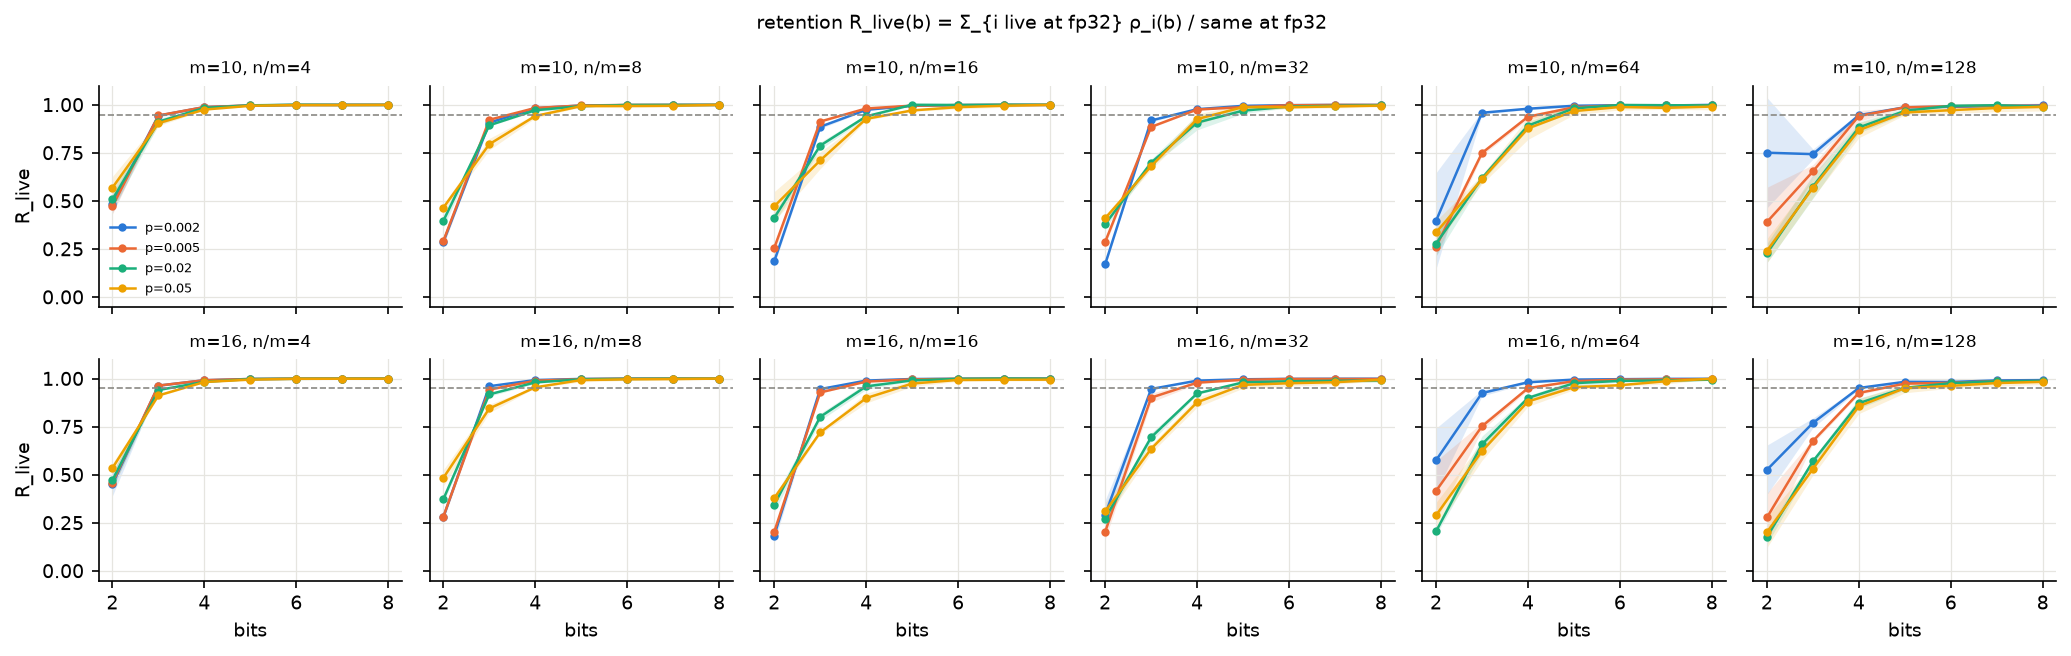
\includegraphics[width=\linewidth]{fig2_Nret_vs_bits.png}
\caption{E1 retention curves for every cell.}\end{figure}
\begin{figure}[h]\centering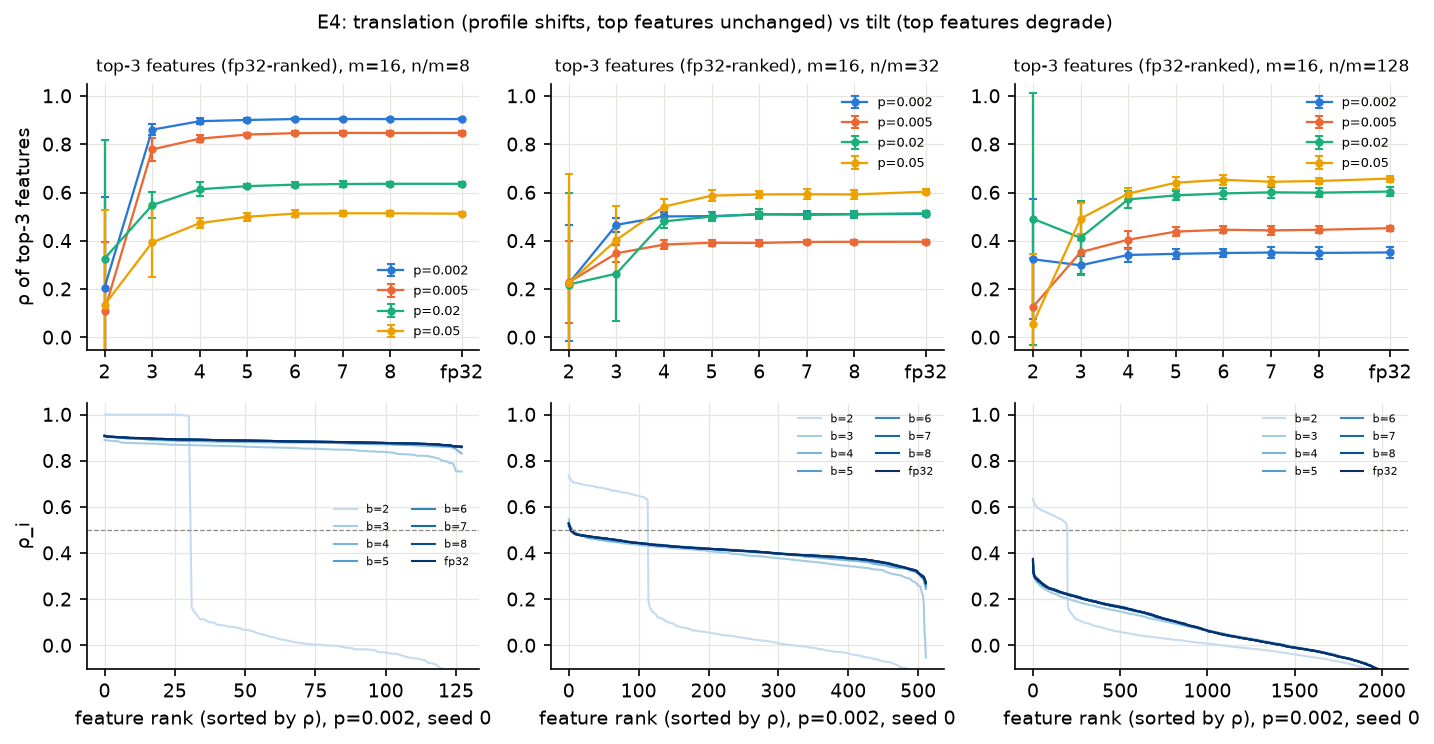
\includegraphics[width=\linewidth]{fig4_translation_vs_tilt.png}
\caption{E4: top-3 feature $\rho$ against bit-width and sorted $\rho$ profiles.}\end{figure}
\begin{figure}[h]\centering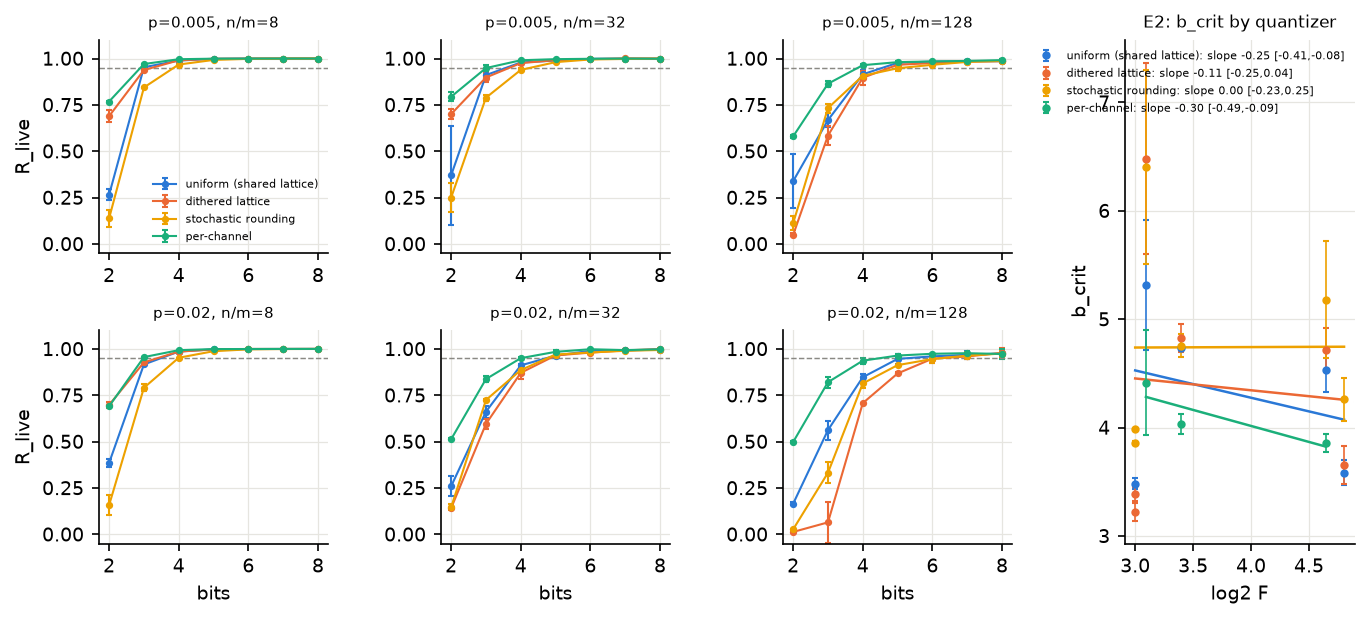
\includegraphics[width=\linewidth]{fig5_lattice.png}
\caption{E2: quantizers under QAT.}\end{figure}
\begin{figure}[h]\centering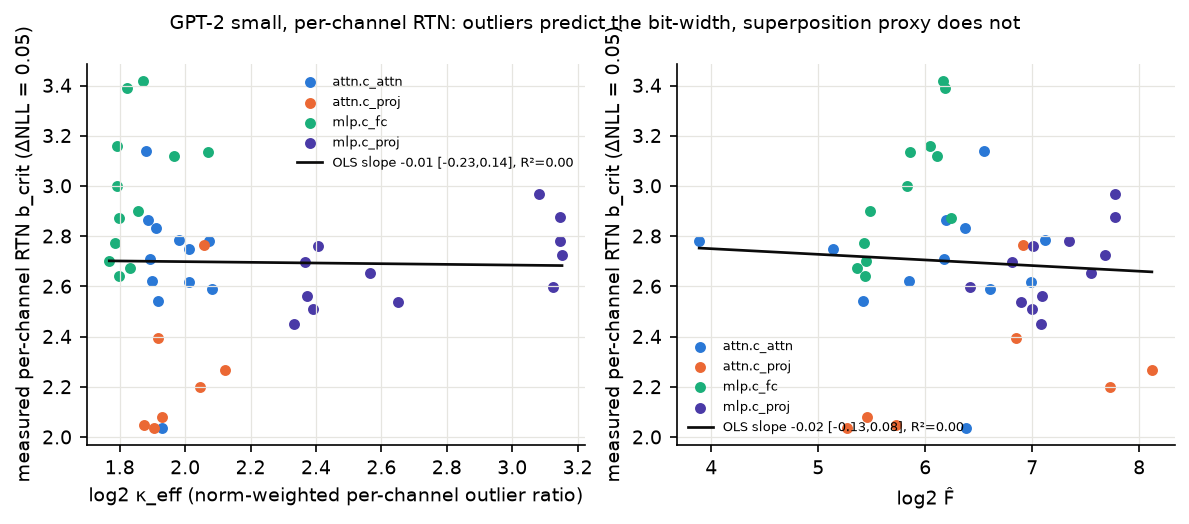
\includegraphics[width=0.8\linewidth]{fig7b_lm_perchannel.png}
\caption{GPT-2 per-channel RTN: all matrices at $2.7\pm0.3$ bits.}\end{figure}
\begin{figure}[h]\centering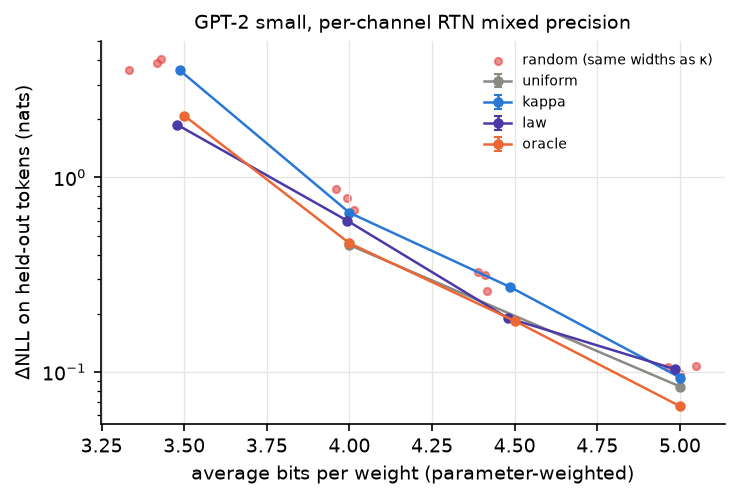
\includegraphics[width=0.6\linewidth]{fig9_mixed_precision.png}
\caption{Mixed precision on GPT-2 small (Table~\ref{tab:mixed}).}\end{figure}

\section{Declaration of LLM and agent usage}
The experiments, analysis code and first drafts of this paper were implemented and executed by an AI coding agent
(Claude Code) under the direction of the author, following a written, preregistered experimental plan; the author
specified the hypotheses, decision rules and controls, reviewed every analysis choice recorded in the deviations log, and
verified the reported numbers against the raw results. This is a non-standard component of the methodology and is
declared per the NeurIPS 2026 policy.

% checklist omitted for the workshop submission (main-track requirement only); re-add \section*{NeurIPS Paper Checklist}
\begin{enumerate}
\item {\bf Claims} \\ Question: Do the main claims made in the abstract and introduction accurately reflect the paper's contributions and scope? \\ Answer: \answerYes{} \\ Justification: Every number in the abstract and contribution list is reported with its CI or $R^2$ in Sec.~3 and App.~C, including the preregistered predictions that failed.
\item {\bf Limitations} \\ Question: Does the paper discuss the limitations of the work performed by the authors? \\ Answer: \answerYes{} \\ Justification: Sec.~5 (single tied layer, criterion-dependent $\sigma^*$, crude superposition proxy, one LM/corpus/SAE layer, sub-unit $\kappa$ slope, metric change from the preregistration).
\item {\bf Theory assumptions and proofs} \\ Question: For each theoretical result, does the paper provide the full set of assumptions and a complete (and correct) proof? \\ Answer: \answerNA{} \\ Justification: The derivations are heuristic scaling arguments with their assumptions stated (unit live columns, Welch-bound interference, uniform residual); no theorem is claimed and the paper tests the predictions empirically.
\item {\bf Experimental result reproducibility} \\ Question: Does the paper fully disclose all the information needed to reproduce the main experimental results? \\ Answer: \answerYes{} \\ Justification: App.~A--B give model, training, quantizer, metric, data, SAE and evaluation details; the preregistration and all per-model results accompany the code.
\item {\bf Open access to data and code} \\ Question: Does the paper provide open access to the data and code? \\ Answer: \answerYes{} \\ Justification: Anonymized code, preregistration, deviation log and per-model result tables are provided as supplementary material and will be released publicly; GPT-2, WikiText-2 and the SAE are public.
\item {\bf Experimental setting/details} \\ Question: Does the paper specify all the training and test details? \\ Answer: \answerYes{} \\ Justification: App.~A (optimizer, schedule, batch, steps, initialisation, evaluation sample counts) and App.~B (token budgets, offsets, thresholds, SAE conventions).
\item {\bf Experiment statistical significance} \\ Question: Does the paper report error bars or other appropriate information about statistical significance? \\ Answer: \answerYes{} \\ Justification: Seed SDs on every toy point, seed-bootstrap 95\,\% CIs on every slope, matrix-bootstrap CIs and $R^2$ for GPT-2 regressions, paired SEMs for quantizer contrasts.
\item {\bf Experiments compute resources} \\ Question: Does the paper provide sufficient information on the computer resources? \\ Answer: \answerYes{} \\ Justification: App.~A: about four GPU-hours on one 24\,GB M-series laptop for all experiments.
\item {\bf Code of ethics} \\ Question: Does the research conform with the NeurIPS Code of Ethics? \\ Answer: \answerYes{} \\ Justification: Public models and data only; no human subjects.
\item {\bf Broader impacts} \\ Question: Does the paper discuss both potential positive and negative societal impacts? \\ Answer: \answerNA{} \\ Justification: Foundational work on when quantization erases representations; it can make compression more predictable and has no direct path to misuse.
\item {\bf Safeguards} \\ Question: Does the paper describe safeguards for responsible release of high-risk assets? \\ Answer: \answerNA{} \\ Justification: No models or datasets are released.
\item {\bf Licenses for existing assets} \\ Question: Are the creators of assets properly credited and licenses respected? \\ Answer: \answerYes{} \\ Justification: GPT-2 (MIT, via Hugging Face), WikiText-2 (CC BY-SA 3.0), the GPT-2 SAEs of \cite{bloom2024sae} (public release), all cited.
\item {\bf New assets} \\ Question: Are new assets well documented? \\ Answer: \answerYes{} \\ Justification: The code base ships with a README, tests and a per-experiment registry.
\item {\bf Crowdsourcing and research with human subjects} \\ Answer: \answerNA{} \\ Justification: None.
\item {\bf Institutional review board (IRB) approvals} \\ Answer: \answerNA{} \\ Justification: No human subjects.
\item {\bf Declaration of LLM usage} \\ Question: Does the paper describe the usage of LLMs if it is an important, original, or non-standard component of the core methods? \\ Answer: \answerYes{} \\ Justification: App.~E declares that an AI coding agent implemented and executed the experiments and analysis under the authors' direction and preregistered plan.
\end{enumerate}
 for a main-track version
\end{document}
